\documentclass[conference]{IEEEtran}
\IEEEoverridecommandlockouts
% The preceding line is only needed to identify funding in the first footnote. If that is unneeded, please comment it out.
\usepackage{cite}
\usepackage{amsmath,amssymb,amsfonts}
\usepackage{algorithmic}
\usepackage{graphicx}
\usepackage{textcomp}
\usepackage{stmaryrd}
\usepackage{verbatim}
\usepackage[]{mdframed}
\usepackage{setspace}
\setstretch{1.5}
\newcommand{\BibTeX}{\textrm{B \kern -.05em \textsc{i \kern -.025em b} \kern -.08em
T \kern -.1667em \lower .7ex \hbox{E} \kern -.125emX}}
\begin{document}

\title{Symmetric Encryption of Audio \\ via Chaotic Neural Networks}

\author{\IEEEauthorblockN{1\textsuperscript{st} Patrick Pfenning}
\IEEEauthorblockA{\textit{School of Computing and Data Science} \\
\textit{Wentworth Institute of Technology}\\
Boston, MA \\
pfenningp@wit.edu}
}

\maketitle

\begin{abstract}
This paper focuses on developing a new algorithm for encrypting audio files symmetrically using a Chaotic Neural Network (CNN).
Said algorithm is benchmarked for its efficiency and effectiveness against another symmetric algorithm Advanced Encryption Standard (AES).
The intent of each layer is to iterate a chosen chaotic map, which can be used to generate pseudo-random arrays.
These arrays are transformed into bitmaps which are used to encrypt files using Waveform Audio File Format.
The results show that the proposed algorithm is more effective than AES in terms of encryption strength, but falls well short in computational efficiency.
\end{abstract}

\begin{IEEEkeywords}
chaos, encryption, audio, neural networks, pseudo-random, symmetric-key, lorenz, logistic, henon, ikeda
\end{IEEEkeywords}

\section{Introduction}\label{sec:introduction}
The world we live in has become wildly dependent on the fast transfer of information.
Everything, from our work and education to our entertainment and social life, often requires the internet as a medium.
With this abundance of information, how can one ensure that their personal data remains private to bad actors?
Enter the field of encryption, the process of encoding information.
Encryption allows one to take a plaintext message we wish to transmit and transform it into a ciphertext.
This ciphertext is illegible to those who do not have a \textit{key}.

Most modern encryption processes create a \textit{psuedo-random} key via a defined algorithm.
These algorithms can be broken into two schemes: \textbf{Symmetric-key Encryption} and \textbf{Public-key Encryption.}
Symmetric-key Encryption algorithms create a single secret key which both the sender and receiver have.
This key is used to both encrypt and decrypt the message.
The security of this method directly depends on the holders of the key as anyone who has it can read the cipher.
Public-key Encryption algorithms require the message receiver to generate both a public and private key.
The receiver shares the public key with the trusted sender who uses it to encrypt a message.
The message is sent to the receiver where the private key is used to decrypt it.
Because the private key is the only way to decipher the message, public-keys can be shared with impunity.
Though both methods do nothing to prevent the cipher from being intercepted by a third party, if the algorithm is strong enough, it should be illegible.

Billions of packets of information flow throughout the internet on a daily basis.
The larger the packet, the longer the encryption will take.
In this paper, we will develop our own algorithm to encrypt several audio files of varying sizes.
The aforementioned algorithm will be developed using what is known as a \textbf{Chaotic Neural Network} (CNN).
This algorithm will be symmetric similar to \textbf{Advanced Encryption Standard} (AES).
This algorithm will be benchmarked for both efficiency and effectiveness against one symmetric-key method, .

\section{Literature Review}\label{sec:literature-review}
\subsection{\textbf{Chaos: An Introduction to Dynamical Systems}~\cite{Alligood}}\label{subsec:chaos:-an-introduction-to-dynamical-systems}

Alligood provides an excellent course in the study of such dynamical systems.
She successfully explains chaotic phenomena in nature using Linear Algebra, Differential Equations and Numeric Analysis.
The book defines chaos as a field of study while introducing the idea of chaotic maps.
These maps are recursive in nature, and are highly sensitive to initial conditions.
Each iteration is mapped to a new phase-space for which the rate of separation of points in the sequence is directly related to the system's Lyapunov Exponents.
There is one exponent for each degree of freedom the chosen system has.
The scalar value of the exponent determines how the basis stretch ($LE > 1$) or shrink ($LE < 1$).
Sequences created by such maps, though deterministic, can be unstable.
These unstable sequences are known as chaotic orbits.
This instability is statistically indistinguishable in nature to randomness, making them ideal candidates for providinging repeatable pseudo-random arrays.

\subsection{\textbf{A Review on Applications of Chaotic Maps in Pseudo-Random Number Generators and Encryption}~\cite{Naik2022}}\label{subsec:a-review-on-applications-of-chaotic-maps-in-pseudo-random-number-generators-and-encryption}

In 2019 Naik and Singh gave a detailed review of Chaotic Neural Networks applications for encryption.
The key aspect, as in many of the papers in this section is the creation of a viable generator.
One way chaotic maps are used to generate a sequence of length \textbf{N}, which is equal to the byte-length of the plaintext file.
These values are then converted to binary and one byte are taken from each value, often the first byte after the decimal point.
This sequence is then reshaped to match the dimensions of the file being encrypted.
The resulting matrices are then XORed with the original file masking the data.
If we preform this action a second time, we will revert to the original data.
This is extremely useful for the decryption process.

This paper also goes through another chaotic tool, diffusion, the act of swapping indices.
The Arnold Cat Map (ACM)~\cite{Naik2022} provides an efficient way to diffuse desired file prior to encrypting, but is most often used for image encryption only.
After several iterations of this map on a matrix the original data is unrecognizable.
It should be noted that orbits of ACM are finite, therefore if the map is iterated to the length of the orbit, all diffusion will be undone.

The largest takeaway of this paper is the review of an audio encryption model using sequences from the Henon and Tent maps.
Said sequences are XORed to create a secret key.
This secret key is then XORed with the audio file to encrypt.
Their correlation coefficient between the plain and ciphered files were as low as 0.0014 with entropy was as high as 7.9995.

\subsection{\textbf{Comparison of Cryptography by Chaotic Neural Network and by AES}\cite{Skovajsova2019}}\label{subsec:comparison-of-cryptography-by-chaotic-neural-network-and-by-aes}

This 2019 paper by Skovajsová~ gives a step by step explanation of how AES encryption works and compares it to a prebuilt CNN\@.
Both algorithms were tested on five random images of each of the following sizes: 512b, 1024b, 2048b, 3KB, 30KB and 3MB\@.
For both ciphering and deciphering, the CNN significantly outperformed the AES model in terms of speed.
The ciphertext created by both models were identical in size to the plaintext file, showing no degradation of information.
It was noted that the CNN used here was a Hopfield network that 1D chaotic maps for its neural weights.
1D maps are much faster for generation, but only require a single initial value.
If this initial condition is found by a bad actor, the algorithm will be broken.
To counteract this, we will be building multiple layer networks of varying dimensionality, each requiring unique sets initial conditions.

\section{Methodology}\label{sec:methodology}

\subsection{Generalization}\label{subsec:generalization}

Suppose there exists some audio file $A$ which we wish to encrypt with our cipher\@.
We first transform $A \rightarrow A^\prime$, such that $A^\prime$ is the matrix containing the header bytes of $A$~\cite{app112110190}.
We now define $N$ to be byte length of $A^\prime$.

We now supply $N$ as a global parameter of our network.
Networks layers are a chosen chaotic map with a unique initial conditions corresponding to:

\begin{mdframed}
\begin{enumerate}
    \item The chosen parameters of the map.
    \item Input variable for each dimension of the map.
    \item Some integer $k$ defining the number of iterations to remove from the generator.
    \item The byte-length $N$, the desired length of our cipher.
\end{enumerate}
\end{mdframed}

For each layer we plug in our parameters, supply our input variables and iterate the map $k+N$ times.
This results in a matrix $Z_{d \times (k+N)}$ such that $d$ is the dimensionality of our map.
Similar to steps in other papers~\cite{Lokesh,app112110190}, we reduce our matrices using the following transformation:

\begin{equation}\label{eq:bitmap}
    W = \bigoplus^{i} \bigoplus^{j} \big\lfloor \left{|} Z_{(i, j)} \right{|} \times 10^{10} \big\rfloor \mod 2^{b}
\end{equation}

Such that $i$ denotes a hidden layer of our network, and $j$ represents a dimension of the layer's map.
$W$ is the logical XOR to the byte-wise representation of our chaotic outputs, resulting in an array of length ${k+N}$.
Finally, we truncate the first $k$ iterations of $W$ to obtaining our cipher $C$ of length $N$.

$C$ can now be used to find our ciphertext such that $E^\prime=A^\prime \oplus C$.
When the sample rate of $A$ is applied to $E^\prime$, it becomes the encrypted audio file $E$.
Given the properties of the XOR operation, $C$ acts as both our encryption and decryption such that:

\begin{equation}\label{eq:xored}
    A^\prime = A^\prime \oplus C \oplus C = E^\prime \oplus C = A^\prime
\end{equation}

This satisfies the requirements of symmetric key encryption.
Theoretically, this methodology should work for any set of chaotic maps we choose.
Because chaotic maps are psuedo-random in nature, the same map can be used in multiple layers, provided that at least one of the map's parameters and/or input variables differ.
It is important to state that because of how $W$~\eqref{eq:bitmap} is calculated, if two layers are identical they will cancel each other out.
Through the rest of this paper we will develop an algorithm using this methodology with our chosen set of chaotic maps.

\begin{mdframed}
\textbf{NOTE:} It is possible for $A$ may have multiple channels of audio.
In cases such as this, we apply $C$ to each channel individually.
This may also open the door to image encryption in the future.
\end{mdframed}

\subsection{Choosing Our Maps}\label{subsec:choosing-our-maps}

We have chosen audio as our medium for encryption.
For ease of use, we will be using Waveform Audio File Format.
Byte representations of these files can be interpreted as $8$-bit or $16$-bit integers thus fitting our methodology nicely.
We have chosen to develop a network consisting of four hidden layers, each representing their own map.
The first layer we will use is the two-dimensional Hénon Map~\cite{Hamdy}:

\begin{equation}\label{eq:Henon}
\begin{aligned}
    x_{n+1} &= 1 - ax_n^2 + y_n \\
    y_{n+1} &= bx_n
\end{aligned}
\end{equation}

\noindent Chaotic behavior occurs here with parameters $a=0.3$ and $b=1.4$.
Our second layer will also be two-dimensional, the Ikeda Map~\cite{app112110190} :

\begin{equation}\label{eq:Ikeda}
\begin{aligned}
    x_{n+1} &= 1 + u(x_n \cos(t_n) - y_n \sin(t_n))\\
    y_{n+1} &= u(x_n \sin(t_n) + y_n \cos(t_n))\\
    t_{n+1} &= \beta - \frac{\gamma}{1+x_{n+1}^2+y_{n+1}^2}
\end{aligned}
\end{equation}

\noindent Where this system develops a chaotic attractor whenever $u\ge0.6$.
Adding complexity, we turn to the three-dimensional map known as the Lorenz attractor~\cite{Naik2022}.

\begin{equation}\label{eq:Lorenz}
\begin{aligned}
    \frac{dx}{dt} &= \sigma (y - x)\\
    \frac{dy}{dt} &= x (\rho - z) - y\\
    \frac{dz}{dt} &= xy - \beta z
\end{aligned}
\end{equation}

\noindent We will use parameter values $\sigma=10$, $\beta=\frac{8}{3}$ and $\rho=28$.
This map is most famous for \textit{The Butterfly Effect}~\cite{Alligood}.
Finally, we will use the most common chaotic function, the Logistic Map~\cite{Qin2017}:

\begin{equation}\label{eq:Logistic}
    x_{n+1} = r x_n (1 - x_n)
\end{equation}

\noindent Such that $r=4$.
It should be noted that $x_0 \in [0,1]$ for chaotic behavior to occur.

Due to the transitive properties of XOR shown in ~\eqref{eq:xored}, the order of these layers is of no consequence.
In fact, these maps will be calculated in parallel, and then be reduced to $W^\prime$~\eqref{eq:bitmap}.

\section{Key Generation}\label{subsec:key-generation}

\begin{comment}
    chaos_key = {
    'primer': int(np.random.randint(100, 10000, 1)),
    'henon': {"params": dict(zip(["a", "b"], [1.4, 0.3])), "v0": np.random.uniform(0, 100, 2).tolist()},
    'ikeda': {"params": dict(zip(["mu", "beta", "gamma"], [0.7, 0.4, 6])), "v0": np.random.uniform(0, 100, 2).tolist()},
    'lorenz': {"params": dict(zip(["sigma", "beta", "rho"], [10, 8 / 3, 28])), "v0": np.random.uniform(0, 100, 3).tolist()},
    'logistic': {"params": dict(zip(["r"], [4])), "v0": np.random.random(1).tolist()},
}
\end{comment}

\section{Experimentation and Results}\label{sec:experimentation-and-results}

\subsection{Processing Time and Complexity}\label{subsec:processing-time-and-complexity}

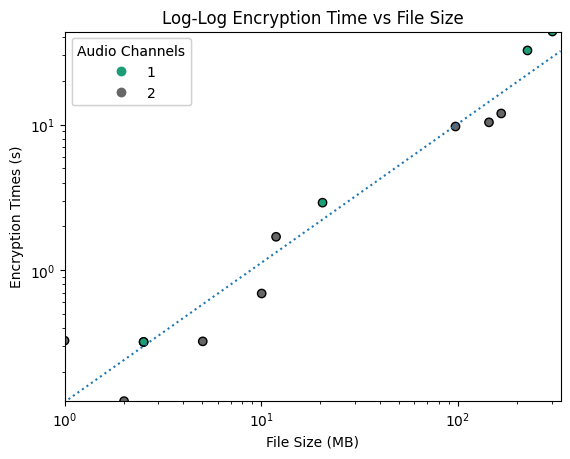
\includegraphics[scale=.35]{figures/loglog}

\subsection{Entropy Analysis}\label{subsec:entropy-analysis}

\begin{comment}
    entropy = 15.96231011061872
\end{comment}


\subsection{Correlation Analysis}\label{subsec:correlation-analysis}

\begin{comment}
    correlation = -0.0004532286205853115
\end{comment}


\subsection{Peak Signal to Noise Ratio}\label{subsec:peak-signal-to-noise-ratio}

\begin{comment}
    psnr_vr_random = -0.00025854809743286467
\end{comment}


\subsection{Key Sensitivity}\label{subsec:key-sensitivity}

\begin{comment}
    inter_psnr = 1.7522768670906752
    inter_corr = -0.0015375314686573802
    k1_primer = 3590
    k2_primer = 3592
\end{comment}

\begin{center}
    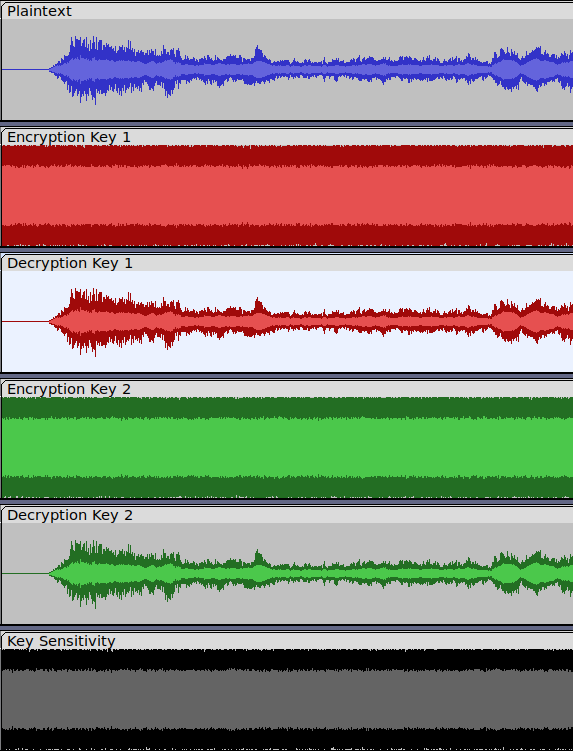
\includegraphics[scale=.25]{figures/MKE}
\end{center}

\subsection{Vulnerability to Attacks}\label{subsec:vulnerability-to-attacks}

\section{Future Work}\label{sec:future-work}

\section{Conclusion}\label{sec:conclusion}

\section{Acknowledgments}\label{sec:acknowledgments}

\bibliographystyle{ieeetr}
\bibliography{bib/bibliography}

\end{document}
